% TODO
% * Namen von Webservices etc mit \emph{Name} hervorheben (möglichst einheitlich, aber IMMER wenn es der Lesbarkeit dient)
% * Gänsefüsse im Text mit \gaensefuesse{}
% * Klassennamen und Objektnamen im Text bitte in \lstinline{}
% * Shift+2 kann unter Window>Preferences>Texlipse>Editor>Smart keys mit der Option {Enable conversion of quotation marks}
%	von ``'' durch abwählen der Option auf " gesetzt werden (wichtig in lstlisting Umgebungen)
\subsubsection{Aufgabe des SAP Connectors}

Die Aufgabe des SAP Connectors besteht darin, die Datenbank im ES Workplace nach einem 
gegebenen Filter zu durchsuchen. Die gefilterten Datensätze werden als Liste zurückgegeben. 

\subsubsection{Aufbau und Programmablauf}

Alle Operationen dienen dazu, Datensätze aus den Datenbanken des ES Workplace auszulesen. Der ES Workplace stellt hierfür 
eine Datenbank mit Testdatensätzen bereit, sowie die erforderlichen Webservices, um eine Verbindung zur Datenbank, 
die Authentifizierung und die Suche selbst durchzuführen. Ein Webservice beschreibt hier eine Software Anwendung, auf 
deren Dienste online über eineals XML basierte Schnittstelle zugegriffen werden kann. Die erforderlichen Webservices 
liegen als XML Dateien vor, werden jedoch zur Verwendung in SIBs als Java Klassen benötigt. Dafür wird Java API for XML Web 
Services verwendet, welches seit Version 1.6  Bestandteil der Java SE ist. Mittels Jax-WS können in der Konsole durch 
einen wsimport Befehl alle benötigten Webservices von XML Dateien in Java Klassen umgewandelt werden. 

Der SAP Connektor erhält ein Objekt vom Typ \lstinline{Contact}. Dieses Objekt enthält die vom Benutzer geforderten Filtereinstellungen 
betreffend Vorname, Nachname, Postleitzahl, Stadt, Straße und Firma. Außerdem wird der Typ nach Kunde, Lieferant und 
Mitarbeiter unterschieden. Dieses Objekt wird verwendet, um in der Datenbank des ES Workplace, nach dem entsprechenden Typ,
Datensätze zu filtern. In Abhängigkeit von der Typbestimmung werden unterschiedliche Webservices ausgeführt:

\textbf{Lieferant}
\begin{itemize}
\item \emph{Find Supplier by Name and Address}
\item \emph{Read Supplier Basic Data}
\end{itemize}

\textbf{Mitarbeiter}
\begin{itemize}
\item \emph{Find Employee by Elements}
\item \emph{Find Employee Address by Employee}
\end{itemize}

\textbf{Kunde}
\begin{itemize}
\item \emph{Find Customer by Elements}
\end{itemize}

Der Programmablauf soll hier am Beispiel des Kundenwebservices beschrieben werden. Anschließend werden die Besonderheiten
bei den Webservices für Mitarbeiter und Lieferant erläutert.

Zunächst müssen die notwendigen Objekte der Klassen des \emph{Webservices Find Customer by Elements} erstellt werden. Mittels
einer Klasse die immer mit dem Schlüsselwort \emph{SERVICE} beginnt, kann ein Objekt erzeugt werden auf dem eine getBinding Methode
ausgeführt wird. Das erstellte Verbindungsobjekt wird dann zu einem Objekt vom Typ Binding Provider gecastet, auf welchem dann
mittels \lstinline{getRequestContext()} Methoden Passwort und Username gesetzt werden können. Für die Authentifizierung ist normalerweise
auch noch eine Webadresse anzugeben, allerdings ist bei den verwendeten Webservices die Adresse der Testdatenbank bereits 
enthalten. Das Verbindungsobjekt verfügt über eine einzige Methode, die ein Objekt mit Suchkriterien übergeben bekommt 
und eine Liste von Suchergebnissen zurückliefert. Die Suchkriterien können mit bereits integrierten set Methoden gesetzt werden,
die Suchergebnisse über get Methoden ausgelesen werden. Anschließend werden die Suchergebnisse als Liste von Kontaktobjekten
zurückgegeben.

Die Webservices \emph{Find Supplier by Name and Address} und \emph{Find Employee by Elements} funktionieren ähnlich, liefern allerdings nur 
einle Liste mit Namen und SAP-IDs. Die SAP-IDs sind eindeutige Nummern, die jedem Datensatz zugeordnet werden. Den Webservices
\emph{Read Supplier Basic Data} und \emph{Find Employee Address by Employee} ist es möglich die fehlenden Adressdaten mit den SAP-IDs 
auszulesen. Dies muss jedoch für jede SAP-ID separat geschehen, also muss für jede SAP-ID von Lieferant und Mitarbeiter der
entsprechende Webservice einzeln aufgerufen werden, die Übergabe einer Liste von IDs ist nicht vorgesehen. Danach können 
die Suchergebnisse auch hier als Liste von Kontaktobjekten zurückgegeben werden.


\subsubsection{Probleme}

Die Verwendung der Webservices des ES Workplace bringt einige Herausforderungen mit sich, was Programmierung und Anwendung
angeht. Die Programmierung wird durch die hohe Anzahl unterschiedlicher Klassen in den Webservices erschwert. Da für jeden
Webservice eigene Objekte erstellt werden müssen, die in den anderen Webservices, selbst bei gleichem Inhalt wie PLZ oder
Stadtname, nicht wiederverwendet werden können, ist eine prozeduraler Programmieransatz die beste Lösung. Eine objektorientierte 
Lösung ist mittels vieler Interfaces, sehr guter Planung und hohem Entwicklungsaufwand zwar auch realisierbar, ob die leicht 
verbesserte Wiederverwendbarkeit den Aufwand allerdings rechtfertigt ist fraglich. Zumal lediglich der Verbindungsaufbau in allen
WSDLs als ähnlich zu betrachten ist, selbst get und set Methoden sind völlig unterschiedlich. Im Beispielcode \ref{lst:codebeispiel}
müssen im Webservice \emph{Find Employee by Elements} erst drei Objekte der inneren Klassen erstellt werden, um im  innersten Objekt 
einen String zuzuweisen und dann die Objekte den Objekten der äußeren Klassen zuzuweisen.

\javalstset{Beispiel für eine einfache Zuweisung}{lst:codebeispiel}
\begin{lstlisting}[float=h!t]

CustomerSelectionByNameAndAddress kundeFilter = new CustomerSelectionByNameAndAddress();
AddressInformation add1 = new AddressInformation();
Address add2            = new Address();
PhysicalAddress add3    = new PhysicalAddress();

add3.setCityName("Hamburg");
add2.setPhysicalAddress(add3);
add1.setAddress(add2);

kundeFilter.setAddressInformation(add1);

\end{lstlisting} 


Ein weiteres Problem stellen die separaten Einzelaufrufe der Webservices für jede ID dar\ref{bild1}. Sollten dem Benutzer keine
vollständigen Informationen vorliegen, könnte ggf. mehr als ein Suchergebnis zurückgegeben werden. Jeder Webserviceaufruf bedingt 
zusätzliche Authentifizierungen und Datenbankzugriffe, die in keinem Verhältnis zum verwendeten Ergebnis stehen.

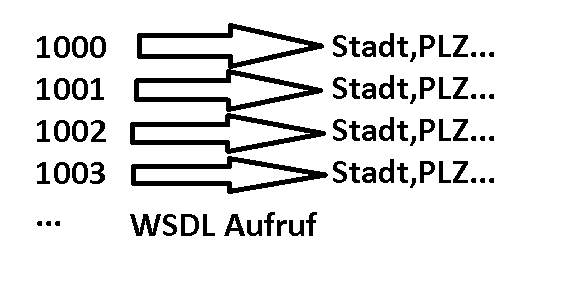
\includegraphics[width=\textheight]{Bilder/presi1.png}{bild1} 


\subsubsection{Ausblick}

Im Folgenden soll eine Lösung für die Mehrfachaufrufe der Webservices beschrieben werden. 

Der erste Webserviceaufruf gibt uns, neben der SAP ID, auch den Namen zurück. Damit hat der Benutzer ein Identifikationsmerkmal, 
welches eine Vorentscheidung, betreffend die zu ladenden Adressdaten, ermöglicht. Wir müssen dem Benutzer jetzt also ermöglichen, nur für 
von ihm ausgewählte Namen die Adressdaten zu laden. Das Graphical User Interface soll nach dem erstem Webserviceaufruf eine 
Liste aller Namen anzeigen, aus welcher der Benutzer einen auswählt. Beim Klick auf einen Namen liefert der Webservice, 
mittels der zugehörigen ID, die Adressdaten zurück \ref{bild2}. Dadurch werden die Authentifizierungen und Datenbankzugriffe reduziert.

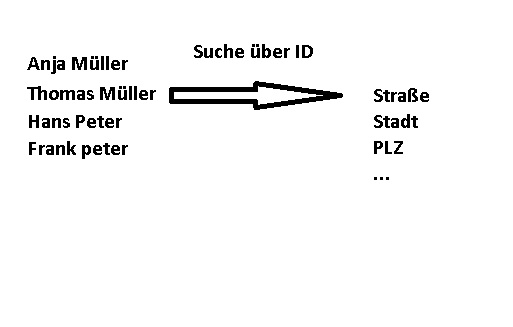
\includegraphics[width=\textheight]{Bilder/presi2.jpg}{bild2}